
% Default to the notebook output style

    


% Inherit from the specified cell style.




    
\documentclass[11pt]{article}

    
    
    \usepackage[T1]{fontenc}
    % Nicer default font (+ math font) than Computer Modern for most use cases
    \usepackage{mathpazo}

    % Basic figure setup, for now with no caption control since it's done
    % automatically by Pandoc (which extracts ![](path) syntax from Markdown).
    \usepackage{graphicx}
    % We will generate all images so they have a width \maxwidth. This means
    % that they will get their normal width if they fit onto the page, but
    % are scaled down if they would overflow the margins.
    \makeatletter
    \def\maxwidth{\ifdim\Gin@nat@width>\linewidth\linewidth
    \else\Gin@nat@width\fi}
    \makeatother
    \let\Oldincludegraphics\includegraphics
    % Set max figure width to be 80% of text width, for now hardcoded.
    \renewcommand{\includegraphics}[1]{\Oldincludegraphics[width=.8\maxwidth]{#1}}
    % Ensure that by default, figures have no caption (until we provide a
    % proper Figure object with a Caption API and a way to capture that
    % in the conversion process - todo).
    \usepackage{caption}
    \DeclareCaptionLabelFormat{nolabel}{}
    \captionsetup{labelformat=nolabel}

    \usepackage{adjustbox} % Used to constrain images to a maximum size 
    \usepackage{xcolor} % Allow colors to be defined
    \usepackage{enumerate} % Needed for markdown enumerations to work
    \usepackage{geometry} % Used to adjust the document margins
    \usepackage{amsmath} % Equations
    \usepackage{amssymb} % Equations
    \usepackage{textcomp} % defines textquotesingle
    % Hack from http://tex.stackexchange.com/a/47451/13684:
    \AtBeginDocument{%
        \def\PYZsq{\textquotesingle}% Upright quotes in Pygmentized code
    }
    \usepackage{upquote} % Upright quotes for verbatim code
    \usepackage{eurosym} % defines \euro
    \usepackage[mathletters]{ucs} % Extended unicode (utf-8) support
    \usepackage[utf8x]{inputenc} % Allow utf-8 characters in the tex document
    \usepackage{fancyvrb} % verbatim replacement that allows latex
    \usepackage{grffile} % extends the file name processing of package graphics 
                         % to support a larger range 
    % The hyperref package gives us a pdf with properly built
    % internal navigation ('pdf bookmarks' for the table of contents,
    % internal cross-reference links, web links for URLs, etc.)
    \usepackage{hyperref}
    \usepackage{longtable} % longtable support required by pandoc >1.10
    \usepackage{booktabs}  % table support for pandoc > 1.12.2
    \usepackage[inline]{enumitem} % IRkernel/repr support (it uses the enumerate* environment)
    \usepackage[normalem]{ulem} % ulem is needed to support strikethroughs (\sout)
                                % normalem makes italics be italics, not underlines
    

    
    
    % Colors for the hyperref package
    \definecolor{urlcolor}{rgb}{0,.145,.698}
    \definecolor{linkcolor}{rgb}{.71,0.21,0.01}
    \definecolor{citecolor}{rgb}{.12,.54,.11}

    % ANSI colors
    \definecolor{ansi-black}{HTML}{3E424D}
    \definecolor{ansi-black-intense}{HTML}{282C36}
    \definecolor{ansi-red}{HTML}{E75C58}
    \definecolor{ansi-red-intense}{HTML}{B22B31}
    \definecolor{ansi-green}{HTML}{00A250}
    \definecolor{ansi-green-intense}{HTML}{007427}
    \definecolor{ansi-yellow}{HTML}{DDB62B}
    \definecolor{ansi-yellow-intense}{HTML}{B27D12}
    \definecolor{ansi-blue}{HTML}{208FFB}
    \definecolor{ansi-blue-intense}{HTML}{0065CA}
    \definecolor{ansi-magenta}{HTML}{D160C4}
    \definecolor{ansi-magenta-intense}{HTML}{A03196}
    \definecolor{ansi-cyan}{HTML}{60C6C8}
    \definecolor{ansi-cyan-intense}{HTML}{258F8F}
    \definecolor{ansi-white}{HTML}{C5C1B4}
    \definecolor{ansi-white-intense}{HTML}{A1A6B2}

    % commands and environments needed by pandoc snippets
    % extracted from the output of `pandoc -s`
    \providecommand{\tightlist}{%
      \setlength{\itemsep}{0pt}\setlength{\parskip}{0pt}}
    \DefineVerbatimEnvironment{Highlighting}{Verbatim}{commandchars=\\\{\}}
    % Add ',fontsize=\small' for more characters per line
    \newenvironment{Shaded}{}{}
    \newcommand{\KeywordTok}[1]{\textcolor[rgb]{0.00,0.44,0.13}{\textbf{{#1}}}}
    \newcommand{\DataTypeTok}[1]{\textcolor[rgb]{0.56,0.13,0.00}{{#1}}}
    \newcommand{\DecValTok}[1]{\textcolor[rgb]{0.25,0.63,0.44}{{#1}}}
    \newcommand{\BaseNTok}[1]{\textcolor[rgb]{0.25,0.63,0.44}{{#1}}}
    \newcommand{\FloatTok}[1]{\textcolor[rgb]{0.25,0.63,0.44}{{#1}}}
    \newcommand{\CharTok}[1]{\textcolor[rgb]{0.25,0.44,0.63}{{#1}}}
    \newcommand{\StringTok}[1]{\textcolor[rgb]{0.25,0.44,0.63}{{#1}}}
    \newcommand{\CommentTok}[1]{\textcolor[rgb]{0.38,0.63,0.69}{\textit{{#1}}}}
    \newcommand{\OtherTok}[1]{\textcolor[rgb]{0.00,0.44,0.13}{{#1}}}
    \newcommand{\AlertTok}[1]{\textcolor[rgb]{1.00,0.00,0.00}{\textbf{{#1}}}}
    \newcommand{\FunctionTok}[1]{\textcolor[rgb]{0.02,0.16,0.49}{{#1}}}
    \newcommand{\RegionMarkerTok}[1]{{#1}}
    \newcommand{\ErrorTok}[1]{\textcolor[rgb]{1.00,0.00,0.00}{\textbf{{#1}}}}
    \newcommand{\NormalTok}[1]{{#1}}
    
    % Additional commands for more recent versions of Pandoc
    \newcommand{\ConstantTok}[1]{\textcolor[rgb]{0.53,0.00,0.00}{{#1}}}
    \newcommand{\SpecialCharTok}[1]{\textcolor[rgb]{0.25,0.44,0.63}{{#1}}}
    \newcommand{\VerbatimStringTok}[1]{\textcolor[rgb]{0.25,0.44,0.63}{{#1}}}
    \newcommand{\SpecialStringTok}[1]{\textcolor[rgb]{0.73,0.40,0.53}{{#1}}}
    \newcommand{\ImportTok}[1]{{#1}}
    \newcommand{\DocumentationTok}[1]{\textcolor[rgb]{0.73,0.13,0.13}{\textit{{#1}}}}
    \newcommand{\AnnotationTok}[1]{\textcolor[rgb]{0.38,0.63,0.69}{\textbf{\textit{{#1}}}}}
    \newcommand{\CommentVarTok}[1]{\textcolor[rgb]{0.38,0.63,0.69}{\textbf{\textit{{#1}}}}}
    \newcommand{\VariableTok}[1]{\textcolor[rgb]{0.10,0.09,0.49}{{#1}}}
    \newcommand{\ControlFlowTok}[1]{\textcolor[rgb]{0.00,0.44,0.13}{\textbf{{#1}}}}
    \newcommand{\OperatorTok}[1]{\textcolor[rgb]{0.40,0.40,0.40}{{#1}}}
    \newcommand{\BuiltInTok}[1]{{#1}}
    \newcommand{\ExtensionTok}[1]{{#1}}
    \newcommand{\PreprocessorTok}[1]{\textcolor[rgb]{0.74,0.48,0.00}{{#1}}}
    \newcommand{\AttributeTok}[1]{\textcolor[rgb]{0.49,0.56,0.16}{{#1}}}
    \newcommand{\InformationTok}[1]{\textcolor[rgb]{0.38,0.63,0.69}{\textbf{\textit{{#1}}}}}
    \newcommand{\WarningTok}[1]{\textcolor[rgb]{0.38,0.63,0.69}{\textbf{\textit{{#1}}}}}
    
    
    % Define a nice break command that doesn't care if a line doesn't already
    % exist.
    \def\br{\hspace*{\fill} \\* }
    % Math Jax compatability definitions
    \def\gt{>}
    \def\lt{<}
    % Document parameters
    \title{Writeup}
    
    
    

    % Pygments definitions
    
\makeatletter
\def\PY@reset{\let\PY@it=\relax \let\PY@bf=\relax%
    \let\PY@ul=\relax \let\PY@tc=\relax%
    \let\PY@bc=\relax \let\PY@ff=\relax}
\def\PY@tok#1{\csname PY@tok@#1\endcsname}
\def\PY@toks#1+{\ifx\relax#1\empty\else%
    \PY@tok{#1}\expandafter\PY@toks\fi}
\def\PY@do#1{\PY@bc{\PY@tc{\PY@ul{%
    \PY@it{\PY@bf{\PY@ff{#1}}}}}}}
\def\PY#1#2{\PY@reset\PY@toks#1+\relax+\PY@do{#2}}

\expandafter\def\csname PY@tok@w\endcsname{\def\PY@tc##1{\textcolor[rgb]{0.73,0.73,0.73}{##1}}}
\expandafter\def\csname PY@tok@c\endcsname{\let\PY@it=\textit\def\PY@tc##1{\textcolor[rgb]{0.25,0.50,0.50}{##1}}}
\expandafter\def\csname PY@tok@cp\endcsname{\def\PY@tc##1{\textcolor[rgb]{0.74,0.48,0.00}{##1}}}
\expandafter\def\csname PY@tok@k\endcsname{\let\PY@bf=\textbf\def\PY@tc##1{\textcolor[rgb]{0.00,0.50,0.00}{##1}}}
\expandafter\def\csname PY@tok@kp\endcsname{\def\PY@tc##1{\textcolor[rgb]{0.00,0.50,0.00}{##1}}}
\expandafter\def\csname PY@tok@kt\endcsname{\def\PY@tc##1{\textcolor[rgb]{0.69,0.00,0.25}{##1}}}
\expandafter\def\csname PY@tok@o\endcsname{\def\PY@tc##1{\textcolor[rgb]{0.40,0.40,0.40}{##1}}}
\expandafter\def\csname PY@tok@ow\endcsname{\let\PY@bf=\textbf\def\PY@tc##1{\textcolor[rgb]{0.67,0.13,1.00}{##1}}}
\expandafter\def\csname PY@tok@nb\endcsname{\def\PY@tc##1{\textcolor[rgb]{0.00,0.50,0.00}{##1}}}
\expandafter\def\csname PY@tok@nf\endcsname{\def\PY@tc##1{\textcolor[rgb]{0.00,0.00,1.00}{##1}}}
\expandafter\def\csname PY@tok@nc\endcsname{\let\PY@bf=\textbf\def\PY@tc##1{\textcolor[rgb]{0.00,0.00,1.00}{##1}}}
\expandafter\def\csname PY@tok@nn\endcsname{\let\PY@bf=\textbf\def\PY@tc##1{\textcolor[rgb]{0.00,0.00,1.00}{##1}}}
\expandafter\def\csname PY@tok@ne\endcsname{\let\PY@bf=\textbf\def\PY@tc##1{\textcolor[rgb]{0.82,0.25,0.23}{##1}}}
\expandafter\def\csname PY@tok@nv\endcsname{\def\PY@tc##1{\textcolor[rgb]{0.10,0.09,0.49}{##1}}}
\expandafter\def\csname PY@tok@no\endcsname{\def\PY@tc##1{\textcolor[rgb]{0.53,0.00,0.00}{##1}}}
\expandafter\def\csname PY@tok@nl\endcsname{\def\PY@tc##1{\textcolor[rgb]{0.63,0.63,0.00}{##1}}}
\expandafter\def\csname PY@tok@ni\endcsname{\let\PY@bf=\textbf\def\PY@tc##1{\textcolor[rgb]{0.60,0.60,0.60}{##1}}}
\expandafter\def\csname PY@tok@na\endcsname{\def\PY@tc##1{\textcolor[rgb]{0.49,0.56,0.16}{##1}}}
\expandafter\def\csname PY@tok@nt\endcsname{\let\PY@bf=\textbf\def\PY@tc##1{\textcolor[rgb]{0.00,0.50,0.00}{##1}}}
\expandafter\def\csname PY@tok@nd\endcsname{\def\PY@tc##1{\textcolor[rgb]{0.67,0.13,1.00}{##1}}}
\expandafter\def\csname PY@tok@s\endcsname{\def\PY@tc##1{\textcolor[rgb]{0.73,0.13,0.13}{##1}}}
\expandafter\def\csname PY@tok@sd\endcsname{\let\PY@it=\textit\def\PY@tc##1{\textcolor[rgb]{0.73,0.13,0.13}{##1}}}
\expandafter\def\csname PY@tok@si\endcsname{\let\PY@bf=\textbf\def\PY@tc##1{\textcolor[rgb]{0.73,0.40,0.53}{##1}}}
\expandafter\def\csname PY@tok@se\endcsname{\let\PY@bf=\textbf\def\PY@tc##1{\textcolor[rgb]{0.73,0.40,0.13}{##1}}}
\expandafter\def\csname PY@tok@sr\endcsname{\def\PY@tc##1{\textcolor[rgb]{0.73,0.40,0.53}{##1}}}
\expandafter\def\csname PY@tok@ss\endcsname{\def\PY@tc##1{\textcolor[rgb]{0.10,0.09,0.49}{##1}}}
\expandafter\def\csname PY@tok@sx\endcsname{\def\PY@tc##1{\textcolor[rgb]{0.00,0.50,0.00}{##1}}}
\expandafter\def\csname PY@tok@m\endcsname{\def\PY@tc##1{\textcolor[rgb]{0.40,0.40,0.40}{##1}}}
\expandafter\def\csname PY@tok@gh\endcsname{\let\PY@bf=\textbf\def\PY@tc##1{\textcolor[rgb]{0.00,0.00,0.50}{##1}}}
\expandafter\def\csname PY@tok@gu\endcsname{\let\PY@bf=\textbf\def\PY@tc##1{\textcolor[rgb]{0.50,0.00,0.50}{##1}}}
\expandafter\def\csname PY@tok@gd\endcsname{\def\PY@tc##1{\textcolor[rgb]{0.63,0.00,0.00}{##1}}}
\expandafter\def\csname PY@tok@gi\endcsname{\def\PY@tc##1{\textcolor[rgb]{0.00,0.63,0.00}{##1}}}
\expandafter\def\csname PY@tok@gr\endcsname{\def\PY@tc##1{\textcolor[rgb]{1.00,0.00,0.00}{##1}}}
\expandafter\def\csname PY@tok@ge\endcsname{\let\PY@it=\textit}
\expandafter\def\csname PY@tok@gs\endcsname{\let\PY@bf=\textbf}
\expandafter\def\csname PY@tok@gp\endcsname{\let\PY@bf=\textbf\def\PY@tc##1{\textcolor[rgb]{0.00,0.00,0.50}{##1}}}
\expandafter\def\csname PY@tok@go\endcsname{\def\PY@tc##1{\textcolor[rgb]{0.53,0.53,0.53}{##1}}}
\expandafter\def\csname PY@tok@gt\endcsname{\def\PY@tc##1{\textcolor[rgb]{0.00,0.27,0.87}{##1}}}
\expandafter\def\csname PY@tok@err\endcsname{\def\PY@bc##1{\setlength{\fboxsep}{0pt}\fcolorbox[rgb]{1.00,0.00,0.00}{1,1,1}{\strut ##1}}}
\expandafter\def\csname PY@tok@kc\endcsname{\let\PY@bf=\textbf\def\PY@tc##1{\textcolor[rgb]{0.00,0.50,0.00}{##1}}}
\expandafter\def\csname PY@tok@kd\endcsname{\let\PY@bf=\textbf\def\PY@tc##1{\textcolor[rgb]{0.00,0.50,0.00}{##1}}}
\expandafter\def\csname PY@tok@kn\endcsname{\let\PY@bf=\textbf\def\PY@tc##1{\textcolor[rgb]{0.00,0.50,0.00}{##1}}}
\expandafter\def\csname PY@tok@kr\endcsname{\let\PY@bf=\textbf\def\PY@tc##1{\textcolor[rgb]{0.00,0.50,0.00}{##1}}}
\expandafter\def\csname PY@tok@bp\endcsname{\def\PY@tc##1{\textcolor[rgb]{0.00,0.50,0.00}{##1}}}
\expandafter\def\csname PY@tok@fm\endcsname{\def\PY@tc##1{\textcolor[rgb]{0.00,0.00,1.00}{##1}}}
\expandafter\def\csname PY@tok@vc\endcsname{\def\PY@tc##1{\textcolor[rgb]{0.10,0.09,0.49}{##1}}}
\expandafter\def\csname PY@tok@vg\endcsname{\def\PY@tc##1{\textcolor[rgb]{0.10,0.09,0.49}{##1}}}
\expandafter\def\csname PY@tok@vi\endcsname{\def\PY@tc##1{\textcolor[rgb]{0.10,0.09,0.49}{##1}}}
\expandafter\def\csname PY@tok@vm\endcsname{\def\PY@tc##1{\textcolor[rgb]{0.10,0.09,0.49}{##1}}}
\expandafter\def\csname PY@tok@sa\endcsname{\def\PY@tc##1{\textcolor[rgb]{0.73,0.13,0.13}{##1}}}
\expandafter\def\csname PY@tok@sb\endcsname{\def\PY@tc##1{\textcolor[rgb]{0.73,0.13,0.13}{##1}}}
\expandafter\def\csname PY@tok@sc\endcsname{\def\PY@tc##1{\textcolor[rgb]{0.73,0.13,0.13}{##1}}}
\expandafter\def\csname PY@tok@dl\endcsname{\def\PY@tc##1{\textcolor[rgb]{0.73,0.13,0.13}{##1}}}
\expandafter\def\csname PY@tok@s2\endcsname{\def\PY@tc##1{\textcolor[rgb]{0.73,0.13,0.13}{##1}}}
\expandafter\def\csname PY@tok@sh\endcsname{\def\PY@tc##1{\textcolor[rgb]{0.73,0.13,0.13}{##1}}}
\expandafter\def\csname PY@tok@s1\endcsname{\def\PY@tc##1{\textcolor[rgb]{0.73,0.13,0.13}{##1}}}
\expandafter\def\csname PY@tok@mb\endcsname{\def\PY@tc##1{\textcolor[rgb]{0.40,0.40,0.40}{##1}}}
\expandafter\def\csname PY@tok@mf\endcsname{\def\PY@tc##1{\textcolor[rgb]{0.40,0.40,0.40}{##1}}}
\expandafter\def\csname PY@tok@mh\endcsname{\def\PY@tc##1{\textcolor[rgb]{0.40,0.40,0.40}{##1}}}
\expandafter\def\csname PY@tok@mi\endcsname{\def\PY@tc##1{\textcolor[rgb]{0.40,0.40,0.40}{##1}}}
\expandafter\def\csname PY@tok@il\endcsname{\def\PY@tc##1{\textcolor[rgb]{0.40,0.40,0.40}{##1}}}
\expandafter\def\csname PY@tok@mo\endcsname{\def\PY@tc##1{\textcolor[rgb]{0.40,0.40,0.40}{##1}}}
\expandafter\def\csname PY@tok@ch\endcsname{\let\PY@it=\textit\def\PY@tc##1{\textcolor[rgb]{0.25,0.50,0.50}{##1}}}
\expandafter\def\csname PY@tok@cm\endcsname{\let\PY@it=\textit\def\PY@tc##1{\textcolor[rgb]{0.25,0.50,0.50}{##1}}}
\expandafter\def\csname PY@tok@cpf\endcsname{\let\PY@it=\textit\def\PY@tc##1{\textcolor[rgb]{0.25,0.50,0.50}{##1}}}
\expandafter\def\csname PY@tok@c1\endcsname{\let\PY@it=\textit\def\PY@tc##1{\textcolor[rgb]{0.25,0.50,0.50}{##1}}}
\expandafter\def\csname PY@tok@cs\endcsname{\let\PY@it=\textit\def\PY@tc##1{\textcolor[rgb]{0.25,0.50,0.50}{##1}}}

\def\PYZbs{\char`\\}
\def\PYZus{\char`\_}
\def\PYZob{\char`\{}
\def\PYZcb{\char`\}}
\def\PYZca{\char`\^}
\def\PYZam{\char`\&}
\def\PYZlt{\char`\<}
\def\PYZgt{\char`\>}
\def\PYZsh{\char`\#}
\def\PYZpc{\char`\%}
\def\PYZdl{\char`\$}
\def\PYZhy{\char`\-}
\def\PYZsq{\char`\'}
\def\PYZdq{\char`\"}
\def\PYZti{\char`\~}
% for compatibility with earlier versions
\def\PYZat{@}
\def\PYZlb{[}
\def\PYZrb{]}
\makeatother


    % Exact colors from NB
    \definecolor{incolor}{rgb}{0.0, 0.0, 0.5}
    \definecolor{outcolor}{rgb}{0.545, 0.0, 0.0}



    
    % Prevent overflowing lines due to hard-to-break entities
    \sloppy 
    % Setup hyperref package
    \hypersetup{
      breaklinks=true,  % so long urls are correctly broken across lines
      colorlinks=true,
      urlcolor=urlcolor,
      linkcolor=linkcolor,
      citecolor=citecolor,
      }
    % Slightly bigger margins than the latex defaults
    
    \geometry{verbose,tmargin=1in,bmargin=1in,lmargin=1in,rmargin=1in}
    
    

    \begin{document}
    
    
    \maketitle
    
    

    
    \section{\texorpdfstring{\textbf{Traffic Sign
Recognition}}{Traffic Sign Recognition}}\label{traffic-sign-recognition}

\subsection{Writeup}\label{writeup}

The aim of this project is to develop an algorithm using deep learning
convolution neural network to classify traffic signs. The project invols
the following steps.

The goals / steps of this project are the following: * Load the data set
(see below for links to the project data set) * Explore, summarize and
visualize the data set * Design, train and test a model architecture *
Use the model to make predictions on new images * Analyze the softmax
probabilities of the new images * Summarize the results with a written
report

\subsubsection{Rubric Points}\label{rubric-points}

\subsection{\texorpdfstring{Here the project reqirements
\href{https://review.udacity.com/\#!/rubrics/481/view}{rubric points}
are considered individually and described in detail how the
implementation is
done.}{Here the project reqirements rubric points are considered individually and described in detail how the implementation is done.}}\label{here-the-project-reqirements-rubric-points-are-considered-individually-and-described-in-detail-how-the-implementation-is-done.}

\begin{center}\rule{0.5\linewidth}{\linethickness}\end{center}

\subsubsection{Project Files}\label{project-files}

The project files includes the python project code written in jupyter
notebook, input dataset stored in .picle format, traffic sign pictures
downloaded from internet. * Here is a link to the
\href{https://github.com/udacity/CarND-Traffic-Sign-Classifier-Project/blob/master/Traffic_Sign_Classifier.ipynb}{project
code}

\subsubsection{Data Set Summary \&
Exploration}\label{data-set-summary-exploration}

\paragraph{1. Dataset Summary}\label{dataset-summary}

The input data contains three sets of data called the training,
validation and test. Only the training dataset is used for training the
neural network. The proformance of trained network is validated using
the validation dataset. Based on the performance of the network measured
from the training and validation set the parameters of the network are
tuned to acheive maximum possible performance. In the following sections
it is explained in detail how the parameters of the network are tuned.
Finally after tuning of parameters the network is tested with test
dataset.

The summary of the dataset are calculated using python native features
and then the dataset is visualized using matplotlib library. The basic
summary of the dataset follows:

\begin{itemize}
\tightlist
\item
  The size of training set is 34799
\item
  The size of the validation set is 4410
\item
  The size of test set is 12630
\item
  The shape of a traffic sign image is (32, 32, 3)
\item
  The number of unique classes/labels in the data set is 43
\end{itemize}

\paragraph{2. Exploratory visualization of the
dataset.}\label{exploratory-visualization-of-the-dataset.}

The images in the dataset are grouped according its class and the no of
images in each class are plotted as a bar chart in the following
picture.

\begin{figure}
\centering
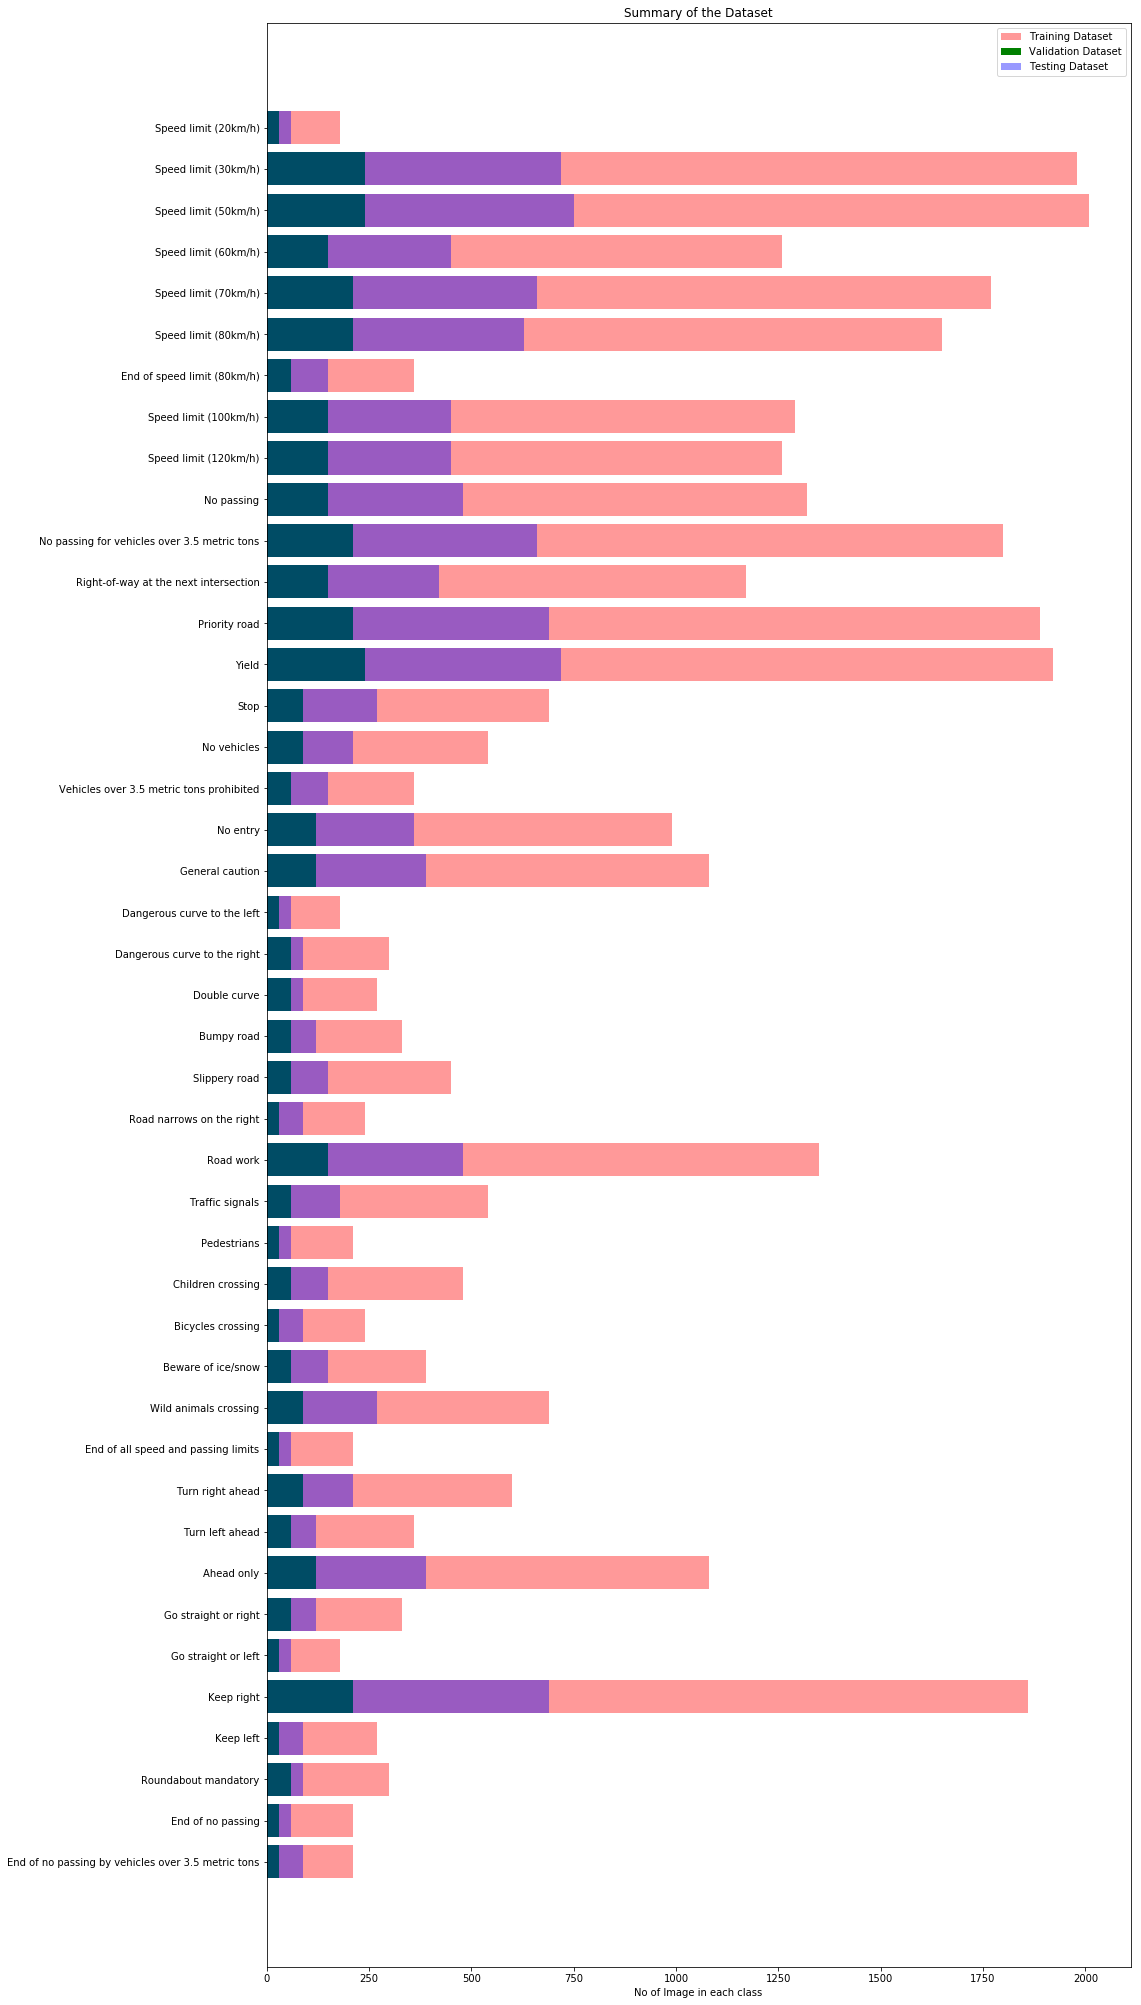
\includegraphics{./BarChart.png}
\caption{alt text}
\end{figure}

The firt thing that can be noted is that the number of images in the
training dataset are greater than validation and test dataset. Large
amount of training data is useful because the network learns better when
it is trained with large dataset. It should also be noted that the
classes such as 'speed limit 50 km/hr' have large amount of data
compared to class such as "Dangerous Curve to the Left". The network
might have difficulty in classifying the traffic signs which have less
data. In such cases it is better to augument the data for such classes.
But in this project this is not done as the network acheived
satisfactory performance.

The datasets have 43 different traffic signs one image in each of the
traffic signs are shown in the picture below.

\begin{figure}
\centering
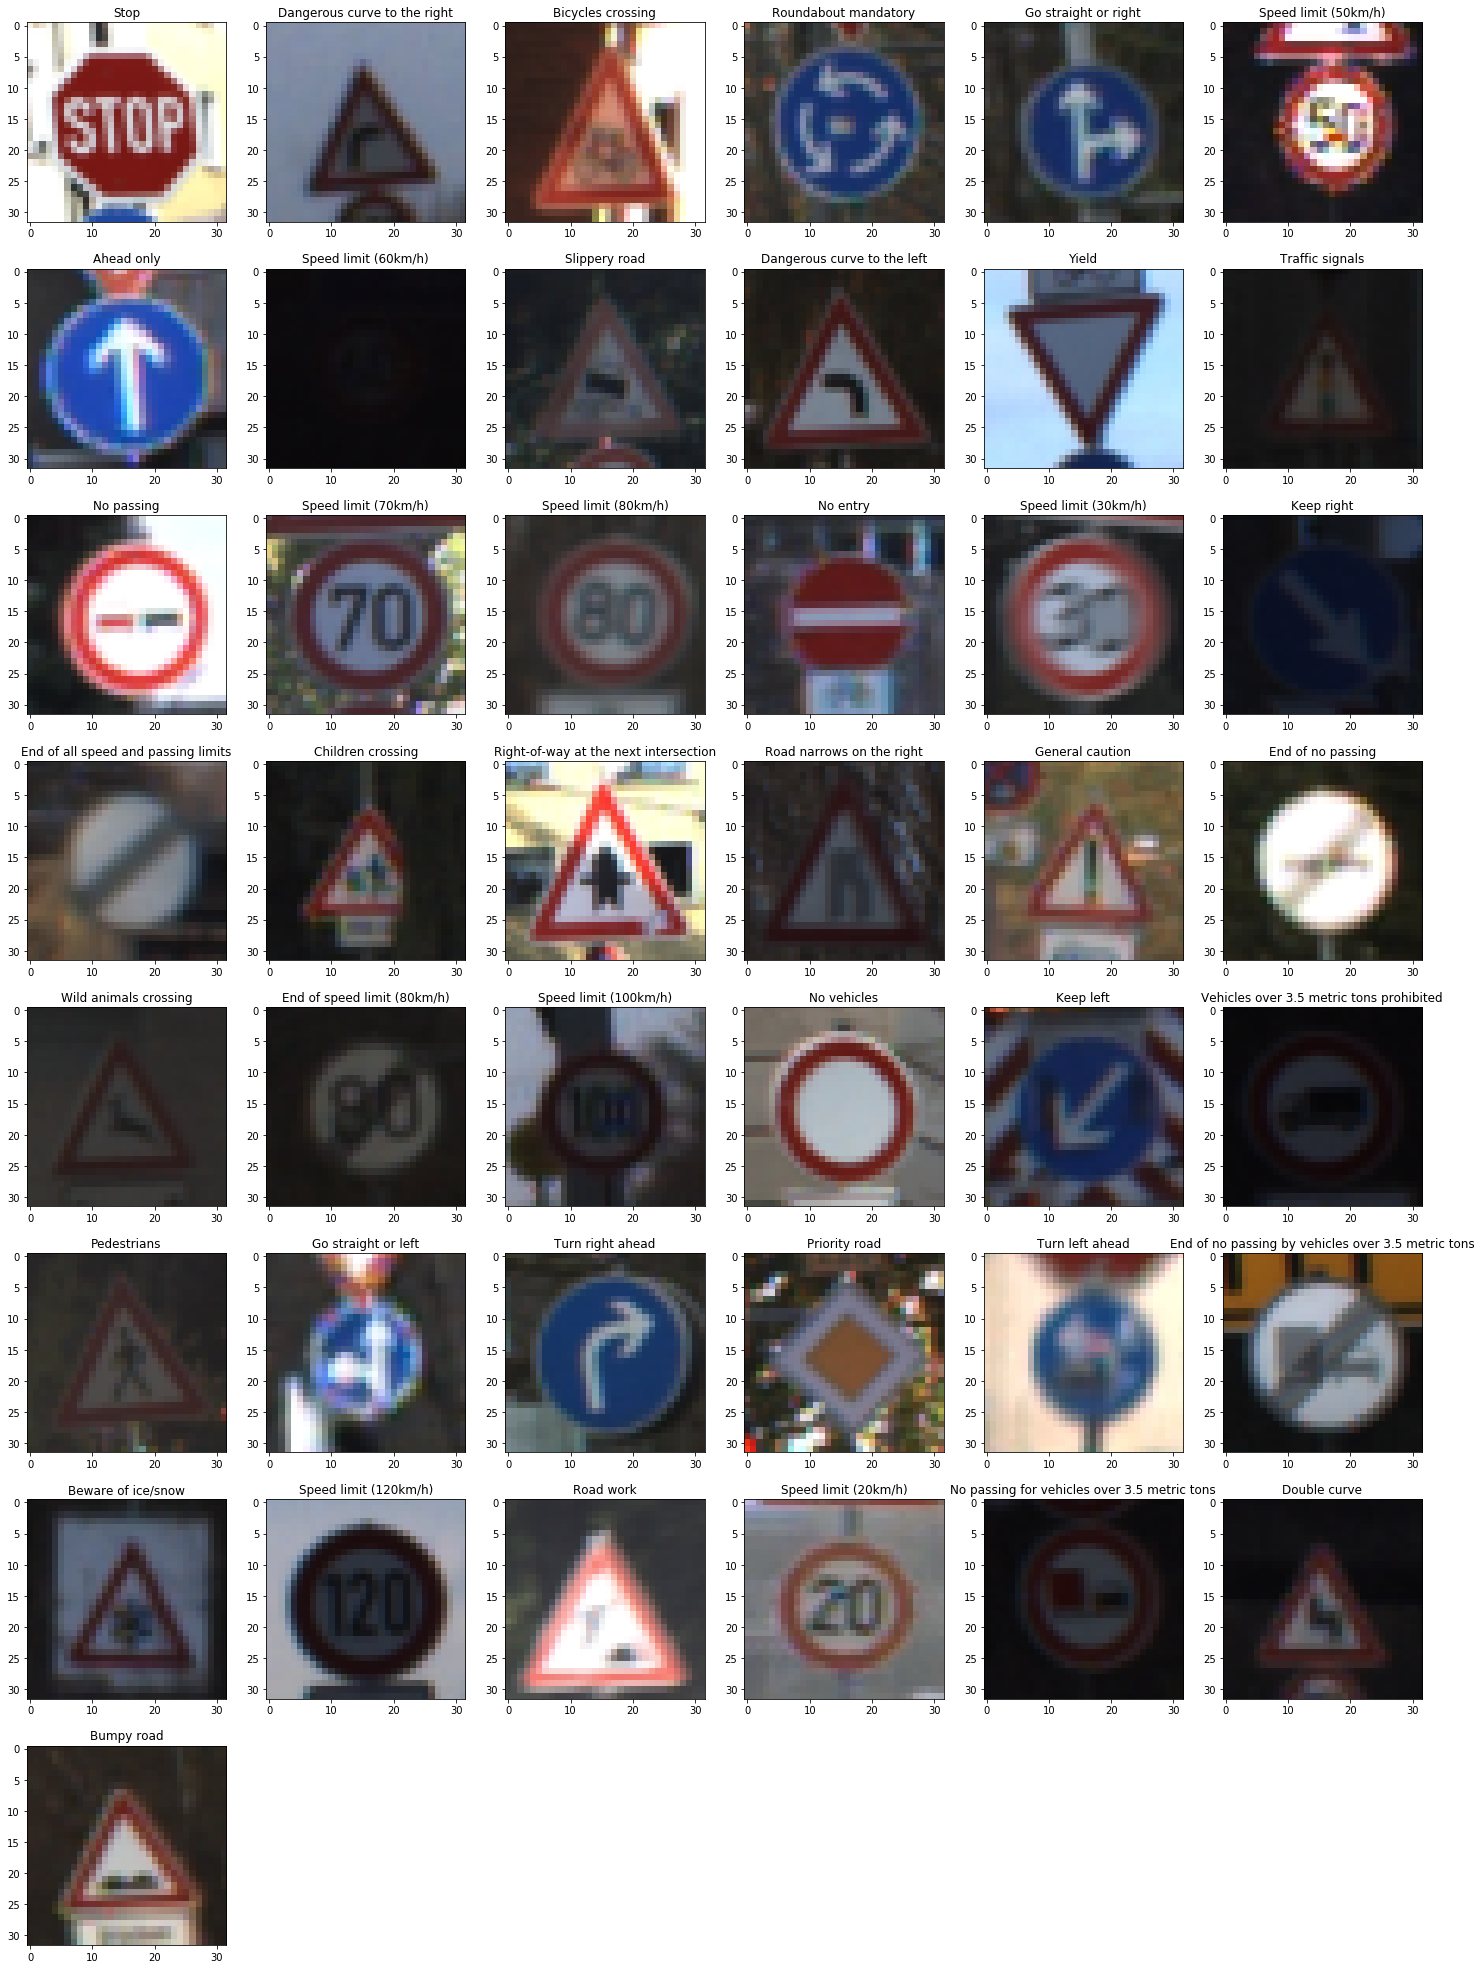
\includegraphics{./TrafficSigns.png}
\caption{alt text}
\end{figure}

\subsubsection{Design and Test a Model
Architecture}\label{design-and-test-a-model-architecture}

\paragraph{1. Preprocessing}\label{preprocessing}

A raw image in RGB format is represented in form of an array of size m x
n x 3 where is m,n are number of pixes along width and height of the
image and 3 represents three channels red,blue and green. Each value in
this array ranges from 0 to 255 for an 8 bit image. The gradient desent
algorithm works better if the input dataset is normalized i.e. the image
has equal variances in both horzontal and vertical directions and zero
mean.

\begin{figure}
\centering
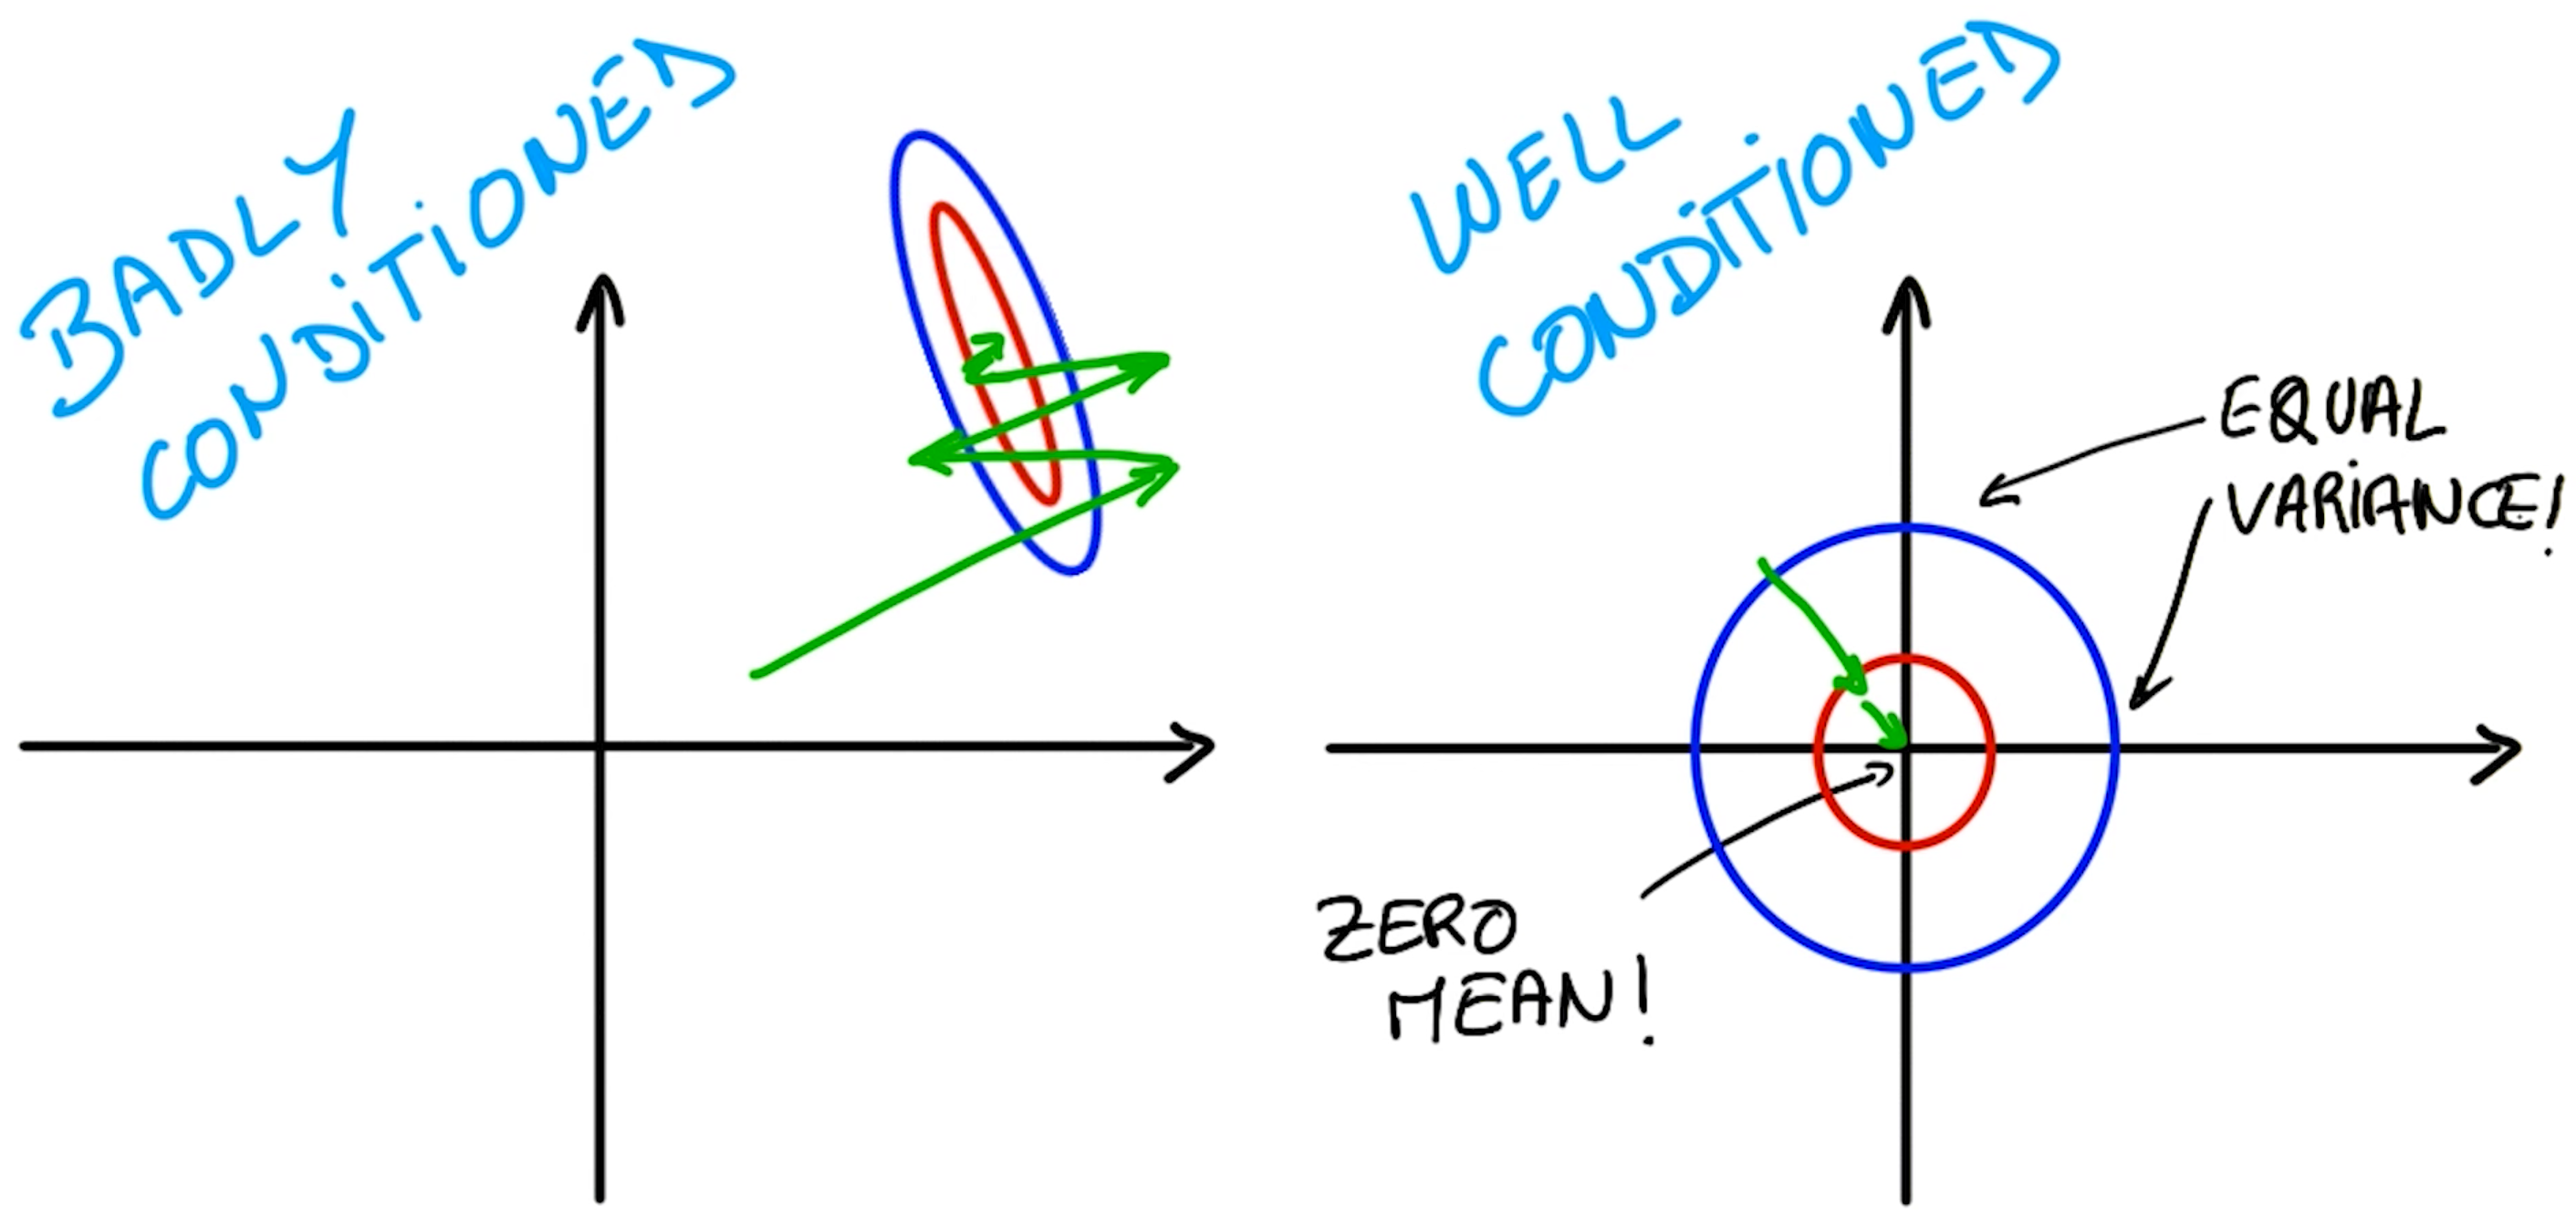
\includegraphics{./mean_variance.png}
\caption{alt text}
\end{figure}

In this project a simpler approach called min-max scaling is used. This
approach scales the input values from 0 to 255 in a 8 bit image to a
values in a given range. The following formula is used to do min-max
scaling.

Min-Max Scaling:
$
X'=a+\{\frac {\left(X-X_{\min }\right)\left(b-a\right)}{X_{\max }-X_{\min }}\}
$

In the above forumla a and b are choosen output range chosen in the
project as 0 and 1. X\_min and X\_max are the minimum and maximum values
of the input data. This formula it simpler because the mean and variance
are avoided and it acheives good performance. The picture below shows
the images before and after normalization.

\begin{figure}
\centering
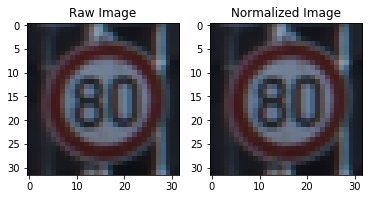
\includegraphics{./Normalization.png}
\caption{alt text}
\end{figure}

This project feeds RGB coloured image to the network as the convolution
neural networks are able to handle 3 channel images and also the colour
information can be useful in classifying the traffic signs as some signs
are in different colours.

\paragraph{2. Model Architecture}\label{model-architecture}

The LeNet architecture is used in this project. The LeNet architecture
is a multi layed neural network architecture which is popularly used to
classify handwritten character recognition. The LeNet architecture
contains two sets of convolution layer and maximul pooling layer
alternatevely followed by three fully connected layer.The convolution
and fully connected layer uses rectified logic units(Relu) for
activation.Finally the output of the final is feed to softmax function
to calculate the probablities of the classes. The following image and
the table shows the LeNet architecture used in this project.

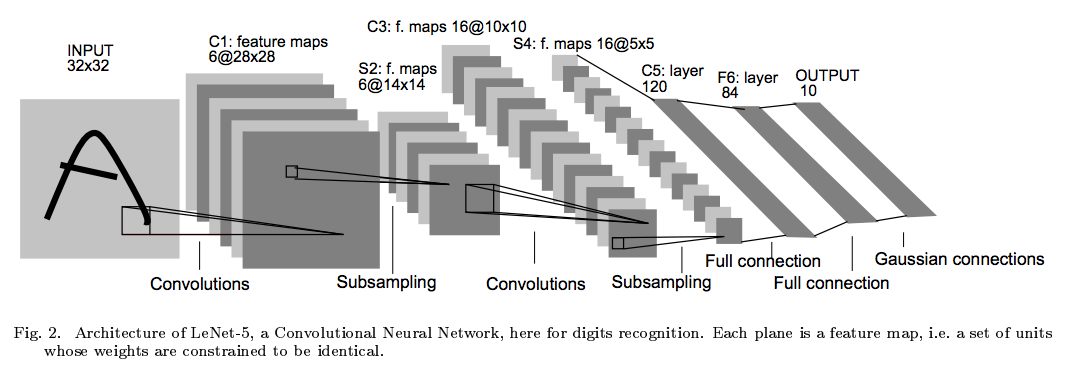
\includegraphics{./LeNet.png} source: Yann Lecunn

\begin{longtable}[]{@{}ll@{}}
\toprule
\begin{minipage}[b]{0.30\columnwidth}\raggedright\strut
Layer\strut
\end{minipage} & \begin{minipage}[b]{0.61\columnwidth}\raggedright\strut
Description\strut
\end{minipage}\tabularnewline
\midrule
\endhead
\begin{minipage}[t]{0.30\columnwidth}\raggedright\strut
Input\strut
\end{minipage} & \begin{minipage}[t]{0.61\columnwidth}\raggedright\strut
32x32x3 RGB image\strut
\end{minipage}\tabularnewline
\begin{minipage}[t]{0.30\columnwidth}\raggedright\strut
1st Convolution\strut
\end{minipage} & \begin{minipage}[t]{0.61\columnwidth}\raggedright\strut
5x5x3x6 filter, 1x1 stride, valid padding, outputs 28x28x6\strut
\end{minipage}\tabularnewline
\begin{minipage}[t]{0.30\columnwidth}\raggedright\strut
RELU\strut
\end{minipage} & \begin{minipage}[t]{0.61\columnwidth}\raggedright\strut
Activation\strut
\end{minipage}\tabularnewline
\begin{minipage}[t]{0.30\columnwidth}\raggedright\strut
Max pooling\strut
\end{minipage} & \begin{minipage}[t]{0.61\columnwidth}\raggedright\strut
2x2 filter, 2x2 stride, outputs 14x14x6\strut
\end{minipage}\tabularnewline
\begin{minipage}[t]{0.30\columnwidth}\raggedright\strut
2nd Convolution\strut
\end{minipage} & \begin{minipage}[t]{0.61\columnwidth}\raggedright\strut
5x5x6x16 filter, 1x1 stride, valid padding, outputs 10x10x16\strut
\end{minipage}\tabularnewline
\begin{minipage}[t]{0.30\columnwidth}\raggedright\strut
RELU\strut
\end{minipage} & \begin{minipage}[t]{0.61\columnwidth}\raggedright\strut
Activation\strut
\end{minipage}\tabularnewline
\begin{minipage}[t]{0.30\columnwidth}\raggedright\strut
Max pooling\strut
\end{minipage} & \begin{minipage}[t]{0.61\columnwidth}\raggedright\strut
2x2 filter, 2x2 stride, outputs 5x5x16\strut
\end{minipage}\tabularnewline
\begin{minipage}[t]{0.30\columnwidth}\raggedright\strut
Flatten\strut
\end{minipage} & \begin{minipage}[t]{0.61\columnwidth}\raggedright\strut
Reshapes the input array into a vector/row matrix,output 5x5x16 =
400\strut
\end{minipage}\tabularnewline
\begin{minipage}[t]{0.30\columnwidth}\raggedright\strut
Fully connected\strut
\end{minipage} & \begin{minipage}[t]{0.61\columnwidth}\raggedright\strut
Flattened array is connected to 120 hidden nodes, weights 400x120,bias
120\strut
\end{minipage}\tabularnewline
\begin{minipage}[t]{0.30\columnwidth}\raggedright\strut
RELU\strut
\end{minipage} & \begin{minipage}[t]{0.61\columnwidth}\raggedright\strut
Activation\strut
\end{minipage}\tabularnewline
\begin{minipage}[t]{0.30\columnwidth}\raggedright\strut
Fully connected\strut
\end{minipage} & \begin{minipage}[t]{0.61\columnwidth}\raggedright\strut
Hidden layer 84 nodes, weights 120x84,bias 84\strut
\end{minipage}\tabularnewline
\begin{minipage}[t]{0.30\columnwidth}\raggedright\strut
RELU\strut
\end{minipage} & \begin{minipage}[t]{0.61\columnwidth}\raggedright\strut
Activation\strut
\end{minipage}\tabularnewline
\begin{minipage}[t]{0.30\columnwidth}\raggedright\strut
Fully connected\strut
\end{minipage} & \begin{minipage}[t]{0.61\columnwidth}\raggedright\strut
Output layer nodes = no. of classes(43), weights 84x43,bias 43\strut
\end{minipage}\tabularnewline
\begin{minipage}[t]{0.30\columnwidth}\raggedright\strut
Softmax\strut
\end{minipage} & \begin{minipage}[t]{0.61\columnwidth}\raggedright\strut
Activation to calulate probablities of the classes\strut
\end{minipage}\tabularnewline
\bottomrule
\end{longtable}

\paragraph{3. Model Training and Solution
Approach}\label{model-training-and-solution-approach}

The model is trained using gradient decent approach to minimize the
cross entropy loss between the softmax predition from the network and
the labels from the input dataset.For the optimizer Adam optimizer is
used,which is an extension of the stocastic gradient desent algorithm.
The adam algorithm is computationally more efficient than the stocastic
gradient desent algorithm. The adam optimizer does not keep the learning
rate constant instead it computes the adaptive learning rates of each of
the parameters based on the first and second order moments of the
gradients. This makes the optimizer more efficient. The details of the
optimizer is out of scope here. The model is trained by feeding the
input datasets in batches, calculating the cross entropy loss and
adapting the weights of the network based on the learning rate. The
whole dataset is feed through the network several times called EPOCHS in
order to train the network better. This leads to several hyper
parameters learning rate, batch size and EPOCHS which have to be tuned
in order to acheive high accuracy. During the traiging of the model
validation dataset is feed through the to evaluate the accuracy of the
network's predictions.The learning rate affects the way the network
learns, higher learning rate means that the weights are changed in
bigger steps this might make the network to overshoot from the taget and
the loss may not be minimized. Lower learning rate reduces the size of
steps the weights are changed and it makes the optimization to converge
better. The batch size also plays similar role as the learning rate as
it is propotional to the number of training steps. If the batch size is
higher the number of training steps is lower and the network may not be
trained to get best possible result. Lowering the batch size increases
the number of iterations in the learning process and thus trains the
network learn better. Like the batch size EPOCHS is also propotional
network's number of learning steps. Higher the EPOCHS the networks
learns better but this can cause the network to overfit the training
dataset. To make to network classify the data with high accurary the
parameters learning rate, batch size and EPOCHS were chosen carfully by
repeated iterations.

Since the training data is used several times in order to train the
network it lead to a problem of overfitting. The network was able to
classify the training data with high accuracy but the it could not
classify the validation data with the same accuracy. To avoid this
problem dropout regularization technique is introduced to the trianing
process, which makes the network more robust. The droput function was
applied on the networks prediction before being fed to the cross entropy
function. The dorpout function randomy drops some of the data in the
networks prediction and doubles the remaining values in order to
maintain the total probablity of the prediction. This forces the network
to become more robust. After application of dropout the network was able
to classify the validation dataset with higher accuracy and closer to
the accuracy of training dataset. The dropout operation adds one more
parameter to the network called the keep probabplity parameter which
ranges from 0 to 1. The keep probablity represents the probabablity of
an element to be kept in the output of the dropout function.

Finally the following parameter values: * Learning Rate = 0.0005 * Batch
Size = 100 * EPOCHS = 40

The final model results were: * training set accuracy of 0.998 *
validation set accuracy of 0.939 * test set accuracy of 0.915

The loss and accurary during the learning process:

\begin{figure}
\centering
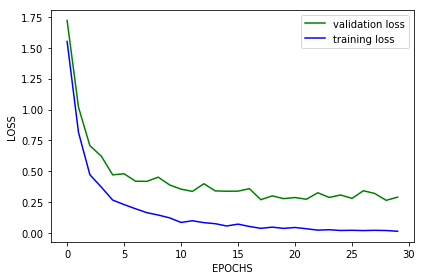
\includegraphics{./Loss.png}
\caption{alt text}
\end{figure}

\begin{figure}
\centering
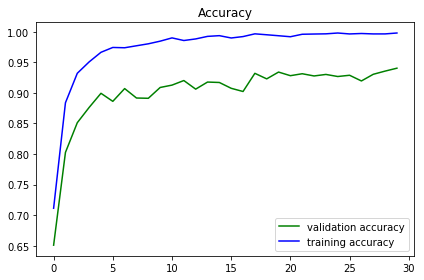
\includegraphics{./Accuracy.png}
\caption{alt text}
\end{figure}

\subsubsection{Test a Model on New
Images}\label{test-a-model-on-new-images}

Some images of the german traffic signs were downloaded from the
internet and these data were feed to the network to be classified. The
network was able to classify 9 out of the 12 signs correctly which is an
accuracy of 0.75.

Traffic signs downloaded from the internet:

\begin{figure}
\centering
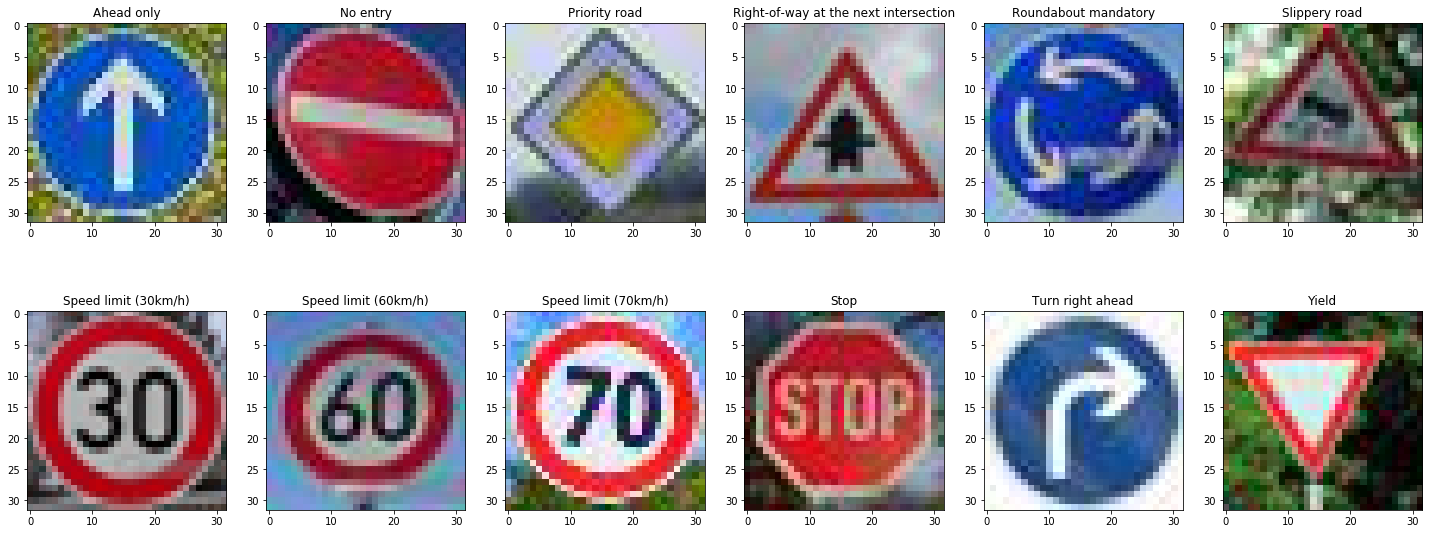
\includegraphics{./TrafficSignsInternetInput.png}
\caption{alt text}
\end{figure}

Prediction made by the network:

\begin{figure}
\centering
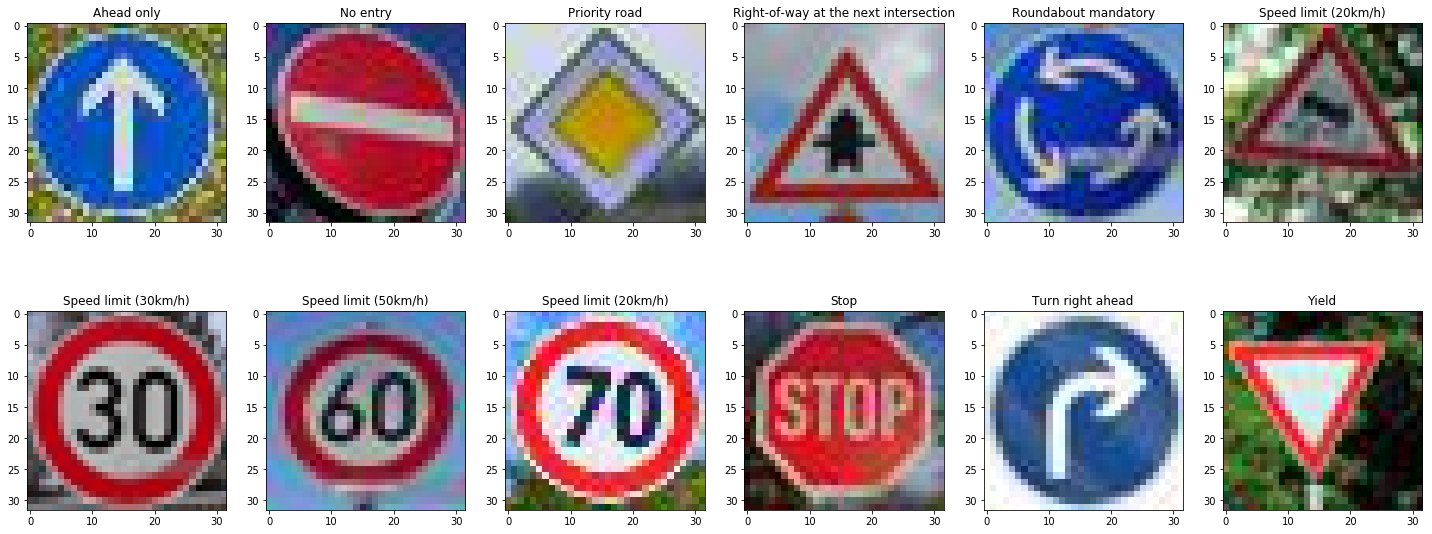
\includegraphics{./TrafficSignsInternetOutput.png}
\caption{alt text}
\end{figure}

The following table shows the top 5 probablities for each of the traffic
signs:

\begin{longtable}[]{@{}ccccccc@{}}
\toprule
\begin{minipage}[b]{0.04\columnwidth}\centering\strut
Image No\strut
\end{minipage} & \begin{minipage}[b]{0.04\columnwidth}\centering\strut
Label\strut
\end{minipage} & \begin{minipage}[b]{0.04\columnwidth}\centering\strut
Highest Probablity\strut
\end{minipage} & \begin{minipage}[b]{0.04\columnwidth}\centering\strut
2nd Highest\strut
\end{minipage} & \begin{minipage}[b]{0.04\columnwidth}\centering\strut
3rd Highest\strut
\end{minipage} & \begin{minipage}[b]{0.04\columnwidth}\centering\strut
4th Highest\strut
\end{minipage} & \begin{minipage}[b]{0.04\columnwidth}\centering\strut
5th Highest\strut
\end{minipage}\tabularnewline
\midrule
\endhead
\begin{minipage}[t]{0.04\columnwidth}\centering\strut
1\strut
\end{minipage} & \begin{minipage}[t]{0.04\columnwidth}\centering\strut
Ahead only\strut
\end{minipage} & \begin{minipage}[t]{0.04\columnwidth}\centering\strut
Ahead only\strut
\end{minipage} & \begin{minipage}[t]{0.04\columnwidth}\centering\strut
Roundabout Mandatory\strut
\end{minipage} & \begin{minipage}[t]{0.04\columnwidth}\centering\strut
Turn Right Ahead\strut
\end{minipage} & \begin{minipage}[t]{0.04\columnwidth}\centering\strut
Go Straight or Right\strut
\end{minipage} & \begin{minipage}[t]{0.04\columnwidth}\centering\strut
Turn Left Ahead\strut
\end{minipage}\tabularnewline
\begin{minipage}[t]{0.04\columnwidth}\centering\strut
\strut
\end{minipage} & \begin{minipage}[t]{0.04\columnwidth}\centering\strut
\strut
\end{minipage} & \begin{minipage}[t]{0.04\columnwidth}\centering\strut
1\strut
\end{minipage} & \begin{minipage}[t]{0.04\columnwidth}\centering\strut
0.000\strut
\end{minipage} & \begin{minipage}[t]{0.04\columnwidth}\centering\strut
0.000\strut
\end{minipage} & \begin{minipage}[t]{0.04\columnwidth}\centering\strut
0.000\strut
\end{minipage} & \begin{minipage}[t]{0.04\columnwidth}\centering\strut
0.000\strut
\end{minipage}\tabularnewline
\begin{minipage}[t]{0.04\columnwidth}\centering\strut
2\strut
\end{minipage} & \begin{minipage}[t]{0.04\columnwidth}\centering\strut
No entry\strut
\end{minipage} & \begin{minipage}[t]{0.04\columnwidth}\centering\strut
No entry\strut
\end{minipage} & \begin{minipage}[t]{0.04\columnwidth}\centering\strut
Yield\strut
\end{minipage} & \begin{minipage}[t]{0.04\columnwidth}\centering\strut
Bicycles Crossing\strut
\end{minipage} & \begin{minipage}[t]{0.04\columnwidth}\centering\strut
No Passing for Vehicles over 3.5 Metric Tons\strut
\end{minipage} & \begin{minipage}[t]{0.04\columnwidth}\centering\strut
Slippery Road\strut
\end{minipage}\tabularnewline
\begin{minipage}[t]{0.04\columnwidth}\centering\strut
\strut
\end{minipage} & \begin{minipage}[t]{0.04\columnwidth}\centering\strut
\strut
\end{minipage} & \begin{minipage}[t]{0.04\columnwidth}\centering\strut
0.589\strut
\end{minipage} & \begin{minipage}[t]{0.04\columnwidth}\centering\strut
0.250\strut
\end{minipage} & \begin{minipage}[t]{0.04\columnwidth}\centering\strut
0.150\strut
\end{minipage} & \begin{minipage}[t]{0.04\columnwidth}\centering\strut
0.008\strut
\end{minipage} & \begin{minipage}[t]{0.04\columnwidth}\centering\strut
0.001\strut
\end{minipage}\tabularnewline
\begin{minipage}[t]{0.04\columnwidth}\centering\strut
3\strut
\end{minipage} & \begin{minipage}[t]{0.04\columnwidth}\centering\strut
Priority road\strut
\end{minipage} & \begin{minipage}[t]{0.04\columnwidth}\centering\strut
Priority road\strut
\end{minipage} & \begin{minipage}[t]{0.04\columnwidth}\centering\strut
End of all speed and passing limits\strut
\end{minipage} & \begin{minipage}[t]{0.04\columnwidth}\centering\strut
Traffic Signals\strut
\end{minipage} & \begin{minipage}[t]{0.04\columnwidth}\centering\strut
End of no passing\strut
\end{minipage} & \begin{minipage}[t]{0.04\columnwidth}\centering\strut
No entry\strut
\end{minipage}\tabularnewline
\begin{minipage}[t]{0.04\columnwidth}\centering\strut
\strut
\end{minipage} & \begin{minipage}[t]{0.04\columnwidth}\centering\strut
\strut
\end{minipage} & \begin{minipage}[t]{0.04\columnwidth}\centering\strut
1\strut
\end{minipage} & \begin{minipage}[t]{0.04\columnwidth}\centering\strut
0.000\strut
\end{minipage} & \begin{minipage}[t]{0.04\columnwidth}\centering\strut
0.000\strut
\end{minipage} & \begin{minipage}[t]{0.04\columnwidth}\centering\strut
0.000\strut
\end{minipage} & \begin{minipage}[t]{0.04\columnwidth}\centering\strut
0.000\strut
\end{minipage}\tabularnewline
\begin{minipage}[t]{0.04\columnwidth}\centering\strut
4\strut
\end{minipage} & \begin{minipage}[t]{0.04\columnwidth}\centering\strut
Right-of-way at the next intersection\strut
\end{minipage} & \begin{minipage}[t]{0.04\columnwidth}\centering\strut
Right-of-way at the next intersection\strut
\end{minipage} & \begin{minipage}[t]{0.04\columnwidth}\centering\strut
Bicycles crossing\strut
\end{minipage} & \begin{minipage}[t]{0.04\columnwidth}\centering\strut
Speed limit(80km/h)\strut
\end{minipage} & \begin{minipage}[t]{0.04\columnwidth}\centering\strut
Beware of ice/snow\strut
\end{minipage} & \begin{minipage}[t]{0.04\columnwidth}\centering\strut
Speed limit (30km/h)\strut
\end{minipage}\tabularnewline
\begin{minipage}[t]{0.04\columnwidth}\centering\strut
\strut
\end{minipage} & \begin{minipage}[t]{0.04\columnwidth}\centering\strut
\strut
\end{minipage} & \begin{minipage}[t]{0.04\columnwidth}\centering\strut
1.000\strut
\end{minipage} & \begin{minipage}[t]{0.04\columnwidth}\centering\strut
0.000\strut
\end{minipage} & \begin{minipage}[t]{0.04\columnwidth}\centering\strut
0.000\strut
\end{minipage} & \begin{minipage}[t]{0.04\columnwidth}\centering\strut
0.000\strut
\end{minipage} & \begin{minipage}[t]{0.04\columnwidth}\centering\strut
0.000\strut
\end{minipage}\tabularnewline
\begin{minipage}[t]{0.04\columnwidth}\centering\strut
5\strut
\end{minipage} & \begin{minipage}[t]{0.04\columnwidth}\centering\strut
Roundabout mandatory\strut
\end{minipage} & \begin{minipage}[t]{0.04\columnwidth}\centering\strut
Roundabout mandatory\strut
\end{minipage} & \begin{minipage}[t]{0.04\columnwidth}\centering\strut
General caution\strut
\end{minipage} & \begin{minipage}[t]{0.04\columnwidth}\centering\strut
Right-of-way at the next intersection\strut
\end{minipage} & \begin{minipage}[t]{0.04\columnwidth}\centering\strut
Children crossing\strut
\end{minipage} & \begin{minipage}[t]{0.04\columnwidth}\centering\strut
Keep right\strut
\end{minipage}\tabularnewline
\begin{minipage}[t]{0.04\columnwidth}\centering\strut
\strut
\end{minipage} & \begin{minipage}[t]{0.04\columnwidth}\centering\strut
\strut
\end{minipage} & \begin{minipage}[t]{0.04\columnwidth}\centering\strut
0.999\strut
\end{minipage} & \begin{minipage}[t]{0.04\columnwidth}\centering\strut
0.001\strut
\end{minipage} & \begin{minipage}[t]{0.04\columnwidth}\centering\strut
0.000\strut
\end{minipage} & \begin{minipage}[t]{0.04\columnwidth}\centering\strut
0.000\strut
\end{minipage} & \begin{minipage}[t]{0.04\columnwidth}\centering\strut
0.000\strut
\end{minipage}\tabularnewline
\begin{minipage}[t]{0.04\columnwidth}\centering\strut
6\strut
\end{minipage} & \begin{minipage}[t]{0.04\columnwidth}\centering\strut
Slippery road\strut
\end{minipage} & \begin{minipage}[t]{0.04\columnwidth}\centering\strut
Speed limit(20km/h)\strut
\end{minipage} & \begin{minipage}[t]{0.04\columnwidth}\centering\strut
No entry\strut
\end{minipage} & \begin{minipage}[t]{0.04\columnwidth}\centering\strut
Dangerous curve to the right\strut
\end{minipage} & \begin{minipage}[t]{0.04\columnwidth}\centering\strut
End of speed limit(80km/h)\strut
\end{minipage} & \begin{minipage}[t]{0.04\columnwidth}\centering\strut
Speed limit(30km/h)\strut
\end{minipage}\tabularnewline
\begin{minipage}[t]{0.04\columnwidth}\centering\strut
\strut
\end{minipage} & \begin{minipage}[t]{0.04\columnwidth}\centering\strut
\strut
\end{minipage} & \begin{minipage}[t]{0.04\columnwidth}\centering\strut
0.958\strut
\end{minipage} & \begin{minipage}[t]{0.04\columnwidth}\centering\strut
0.034\strut
\end{minipage} & \begin{minipage}[t]{0.04\columnwidth}\centering\strut
0.004\strut
\end{minipage} & \begin{minipage}[t]{0.04\columnwidth}\centering\strut
0.002\strut
\end{minipage} & \begin{minipage}[t]{0.04\columnwidth}\centering\strut
0.000\strut
\end{minipage}\tabularnewline
\begin{minipage}[t]{0.04\columnwidth}\centering\strut
7\strut
\end{minipage} & \begin{minipage}[t]{0.04\columnwidth}\centering\strut
Speed limit(30km/h)\strut
\end{minipage} & \begin{minipage}[t]{0.04\columnwidth}\centering\strut
Speed limit(30km/h)\strut
\end{minipage} & \begin{minipage}[t]{0.04\columnwidth}\centering\strut
Speed limit(50km/h)\strut
\end{minipage} & \begin{minipage}[t]{0.04\columnwidth}\centering\strut
Go straingt or right\strut
\end{minipage} & \begin{minipage}[t]{0.04\columnwidth}\centering\strut
Keep right\strut
\end{minipage} & \begin{minipage}[t]{0.04\columnwidth}\centering\strut
End of all speed and passing limits\strut
\end{minipage}\tabularnewline
\begin{minipage}[t]{0.04\columnwidth}\centering\strut
\strut
\end{minipage} & \begin{minipage}[t]{0.04\columnwidth}\centering\strut
\strut
\end{minipage} & \begin{minipage}[t]{0.04\columnwidth}\centering\strut
0.937\strut
\end{minipage} & \begin{minipage}[t]{0.04\columnwidth}\centering\strut
0.062\strut
\end{minipage} & \begin{minipage}[t]{0.04\columnwidth}\centering\strut
0.000\strut
\end{minipage} & \begin{minipage}[t]{0.04\columnwidth}\centering\strut
0.000\strut
\end{minipage} & \begin{minipage}[t]{0.04\columnwidth}\centering\strut
0.000\strut
\end{minipage}\tabularnewline
\begin{minipage}[t]{0.04\columnwidth}\centering\strut
8\strut
\end{minipage} & \begin{minipage}[t]{0.04\columnwidth}\centering\strut
Speed limit(60km/h)\strut
\end{minipage} & \begin{minipage}[t]{0.04\columnwidth}\centering\strut
Speed limit(50km/h)\strut
\end{minipage} & \begin{minipage}[t]{0.04\columnwidth}\centering\strut
Speed limit(60km/h)\strut
\end{minipage} & \begin{minipage}[t]{0.04\columnwidth}\centering\strut
Speed limit(80km/h)\strut
\end{minipage} & \begin{minipage}[t]{0.04\columnwidth}\centering\strut
Speed limit(30km/h)\strut
\end{minipage} & \begin{minipage}[t]{0.04\columnwidth}\centering\strut
Go straight or right\strut
\end{minipage}\tabularnewline
\begin{minipage}[t]{0.04\columnwidth}\centering\strut
\strut
\end{minipage} & \begin{minipage}[t]{0.04\columnwidth}\centering\strut
\strut
\end{minipage} & \begin{minipage}[t]{0.04\columnwidth}\centering\strut
0.718\strut
\end{minipage} & \begin{minipage}[t]{0.04\columnwidth}\centering\strut
0.282\strut
\end{minipage} & \begin{minipage}[t]{0.04\columnwidth}\centering\strut
0.000\strut
\end{minipage} & \begin{minipage}[t]{0.04\columnwidth}\centering\strut
0.000\strut
\end{minipage} & \begin{minipage}[t]{0.04\columnwidth}\centering\strut
0.000\strut
\end{minipage}\tabularnewline
\begin{minipage}[t]{0.04\columnwidth}\centering\strut
9\strut
\end{minipage} & \begin{minipage}[t]{0.04\columnwidth}\centering\strut
Speed limit(70km/h)\strut
\end{minipage} & \begin{minipage}[t]{0.04\columnwidth}\centering\strut
Speed limit(20km/h)\strut
\end{minipage} & \begin{minipage}[t]{0.04\columnwidth}\centering\strut
Bicycles crossing\strut
\end{minipage} & \begin{minipage}[t]{0.04\columnwidth}\centering\strut
Ahead only\strut
\end{minipage} & \begin{minipage}[t]{0.04\columnwidth}\centering\strut
Speed limit(30km/h)\strut
\end{minipage} & \begin{minipage}[t]{0.04\columnwidth}\centering\strut
Go straight or right\strut
\end{minipage}\tabularnewline
\begin{minipage}[t]{0.04\columnwidth}\centering\strut
\strut
\end{minipage} & \begin{minipage}[t]{0.04\columnwidth}\centering\strut
\strut
\end{minipage} & \begin{minipage}[t]{0.04\columnwidth}\centering\strut
0.589\strut
\end{minipage} & \begin{minipage}[t]{0.04\columnwidth}\centering\strut
0.373\strut
\end{minipage} & \begin{minipage}[t]{0.04\columnwidth}\centering\strut
0.033\strut
\end{minipage} & \begin{minipage}[t]{0.04\columnwidth}\centering\strut
0.005\strut
\end{minipage} & \begin{minipage}[t]{0.04\columnwidth}\centering\strut
0.000\strut
\end{minipage}\tabularnewline
\begin{minipage}[t]{0.04\columnwidth}\centering\strut
10\strut
\end{minipage} & \begin{minipage}[t]{0.04\columnwidth}\centering\strut
Stop\strut
\end{minipage} & \begin{minipage}[t]{0.04\columnwidth}\centering\strut
Stop\strut
\end{minipage} & \begin{minipage}[t]{0.04\columnwidth}\centering\strut
Speed limit(30km/h)\strut
\end{minipage} & \begin{minipage}[t]{0.04\columnwidth}\centering\strut
Speed limit(80km/h)\strut
\end{minipage} & \begin{minipage}[t]{0.04\columnwidth}\centering\strut
Priority road\strut
\end{minipage} & \begin{minipage}[t]{0.04\columnwidth}\centering\strut
Speed limit(50km/h)\strut
\end{minipage}\tabularnewline
\begin{minipage}[t]{0.04\columnwidth}\centering\strut
\strut
\end{minipage} & \begin{minipage}[t]{0.04\columnwidth}\centering\strut
\strut
\end{minipage} & \begin{minipage}[t]{0.04\columnwidth}\centering\strut
0.985\strut
\end{minipage} & \begin{minipage}[t]{0.04\columnwidth}\centering\strut
0.014\strut
\end{minipage} & \begin{minipage}[t]{0.04\columnwidth}\centering\strut
0.001\strut
\end{minipage} & \begin{minipage}[t]{0.04\columnwidth}\centering\strut
0.000\strut
\end{minipage} & \begin{minipage}[t]{0.04\columnwidth}\centering\strut
0.000\strut
\end{minipage}\tabularnewline
\begin{minipage}[t]{0.04\columnwidth}\centering\strut
11\strut
\end{minipage} & \begin{minipage}[t]{0.04\columnwidth}\centering\strut
Turn right ahead\strut
\end{minipage} & \begin{minipage}[t]{0.04\columnwidth}\centering\strut
Turn right ahead\strut
\end{minipage} & \begin{minipage}[t]{0.04\columnwidth}\centering\strut
Right-of-the-way at the next intersection\strut
\end{minipage} & \begin{minipage}[t]{0.04\columnwidth}\centering\strut
Beware of ice/snow\strut
\end{minipage} & \begin{minipage}[t]{0.04\columnwidth}\centering\strut
Road narrows on the right\strut
\end{minipage} & \begin{minipage}[t]{0.04\columnwidth}\centering\strut
Double curve\strut
\end{minipage}\tabularnewline
\begin{minipage}[t]{0.04\columnwidth}\centering\strut
\strut
\end{minipage} & \begin{minipage}[t]{0.04\columnwidth}\centering\strut
\strut
\end{minipage} & \begin{minipage}[t]{0.04\columnwidth}\centering\strut
0.623\strut
\end{minipage} & \begin{minipage}[t]{0.04\columnwidth}\centering\strut
0.377\strut
\end{minipage} & \begin{minipage}[t]{0.04\columnwidth}\centering\strut
0.000\strut
\end{minipage} & \begin{minipage}[t]{0.04\columnwidth}\centering\strut
0.000\strut
\end{minipage} & \begin{minipage}[t]{0.04\columnwidth}\centering\strut
0.000\strut
\end{minipage}\tabularnewline
\begin{minipage}[t]{0.04\columnwidth}\centering\strut
12\strut
\end{minipage} & \begin{minipage}[t]{0.04\columnwidth}\centering\strut
Yield\strut
\end{minipage} & \begin{minipage}[t]{0.04\columnwidth}\centering\strut
Yield\strut
\end{minipage} & \begin{minipage}[t]{0.04\columnwidth}\centering\strut
Speed limit(30km/h)\strut
\end{minipage} & \begin{minipage}[t]{0.04\columnwidth}\centering\strut
No vehiclea\strut
\end{minipage} & \begin{minipage}[t]{0.04\columnwidth}\centering\strut
No passing\strut
\end{minipage} & \begin{minipage}[t]{0.04\columnwidth}\centering\strut
Speed limit(60km/h)\strut
\end{minipage}\tabularnewline
\begin{minipage}[t]{0.04\columnwidth}\centering\strut
\strut
\end{minipage} & \begin{minipage}[t]{0.04\columnwidth}\centering\strut
\strut
\end{minipage} & \begin{minipage}[t]{0.04\columnwidth}\centering\strut
1.000\strut
\end{minipage} & \begin{minipage}[t]{0.04\columnwidth}\centering\strut
0.000\strut
\end{minipage} & \begin{minipage}[t]{0.04\columnwidth}\centering\strut
0.000\strut
\end{minipage} & \begin{minipage}[t]{0.04\columnwidth}\centering\strut
0.000\strut
\end{minipage} & \begin{minipage}[t]{0.04\columnwidth}\centering\strut
0.000\strut
\end{minipage}\tabularnewline
\bottomrule
\end{longtable}

The network was not able to classify the traffic signs Slippery Road,
Speed Limit 60km/h and Speed Limit 70km/h. Only around 500 images of
slippery road traffic sign was used during the training, may the
training dataset with more images could be used to train the network or
data augumentaion could be used to improve the networks ability to
classify this sign. If we look at the top probablities for the speed
limit signs the network is not able to classify the digits in the
traffic signs properly. For traffic signs speed limit 60 km/h it
predicts as 70km/h and for speed limit 70km/h it predicts as 20km/h
speed limit. This suggest that the network can be trained more to
improve the classification of similar images. To make the algorithm work
better the traffic sign recognition can be done in two steps, in the
first step the network should be trained to classify the type of road
sign such as speed limits, cautions, directions etc.Then in the second
step the network should classify the specific sign such as speed limit
50km/h, 70km/h etc.


    % Add a bibliography block to the postdoc
    
    
    
    \end{document}
